\documentclass[11pt, a4paper]{article}

% --- UNIVERSAL PREAMBLE BLOCK ---
\usepackage[a4paper, top=2.5cm, bottom=2.5cm, left=2cm, right=2cm]{geometry}
\usepackage{fontspec}
\usepackage[english, bidi=basic, provide=*]{babel}
\babelprovide[import, onchar=ids fonts]{english}
\babelfont{rm}{Noto Sans}

% Additional packages for formatting
\usepackage{parskip}
\usepackage{titlesec}
\usepackage{natbib}
\usepackage{hyperref}
\usepackage{booktabs}
\usepackage{array}
\usepackage{graphicx}
\usepackage{tikz} % Added for workflow diagram

\title{\textbf{A Diachronic Analysis of Gender Neutrality and Contributor Demographics Across Task Continuums on wikiHow}}
\author{Ebha Baxla \\ \textit{School of Liberal Arts (SOLA), Azim Premji University}}
\date{\today}

\begin{document}

\maketitle

\begin{abstract}
Collaborative knowledge platforms serve as vast repositories of human instruction, yet they frequently mirror offline societal and historical gender disparities. This research conducts a diachronic analysis of wikiHow articles to investigate the relationship between contributor demographics and the evolution of gender-neutral language. By mapping articles along four distinct continuums of traditionally gender-coded tasks---ranging from domestic roles and entertainment to occupational fields and governance policy---this study quantifies how the gender distribution of contributors influences the linguistic neutrality of instructional content over time. Utilizing a continuous data extraction pipeline via Google Colab, coupled with composite NLP semantic filters integrating multiple standardized GitHub repositories (e.g., Bolukbasi, WinoBias, Google Jigsaw), the research compiles an expanding database of historical article revisions. Preliminary frameworks suggest that while instructional language trends toward neutrality over time, the rate of this shift is heavily moderated by the dominant gender demographic of the space, highlighting active ``gatekeeping'' effects, the targeted nature of platform vandalism, and extreme demographic shifts (Gender Flips) in specific micro-domains.
\end{abstract}

\vspace{0.5cm}

\section{Introduction}
As Artificial Intelligence systems increasingly rely on scraped internet data for training, understanding the biases embedded within collaborative platforms has become an urgent computational challenge. A central philosophical debate in the study of digital platforms is whether these spaces act as a \textit{mirror}---simply reflecting the offline inequalities of society---or as a \textit{mold}---actively enforcing those disparities by marginalizing minority contributors. 

Offline, sociological data paints a rigid picture of gendered labor. Multinational time-use surveys reveal that daily domestic maintenance tasks represent a stubborn limit to the equal distribution of housework. Even when women transition to flexible self-employment, they predominantly use this flexibility to combine earning with childcare, rather than experiencing a redistribution of domestic labor with male partners. 

Does the digital world mirror this stubborn offline reality? While extensive research has documented the participation gaps on Wikipedia, fewer studies have analyzed the longitudinal evolution of gendered language on instructional platforms like wikiHow. The primary objective of this research is to determine whether female-coded instructional spaces utilize more neutral language than male-coded spaces, and how this dynamic shifts as articles undergo thousands of revisions over decades. 

\section{Literature Review and Theoretical Framework}

\subsection{The Participation Gap and Diachronic Analysis}
The foundation of platform disparity research demonstrates that the gender gap in collaborative contributions is deeply tied to digital literacy (Hargittai \& Shaw, 2015). Methodologically, Suhr and Roth (2024) established that rule-based ``Static List'' classifiers are highly effective for tracking gender-neutral language. To prevent algorithmic bias and ensure a wide-ranging, comprehensive analysis, this study combines multiple standardized, open-source lexicons. This composite approach aggregates the \textit{debiaswe} corpus (Bolukbasi et al., 2016), UCLA's WinoBias occupational dataset, and Meta's Multi-Dimensional Gender Lexicon (MDGender) to form a robust, peer-reviewed linguistic measuring tool.

\subsection{The Domestic and Occupational Axes}
To establish the baseline continuums, it is necessary to examine the division of labor. Time-use survey data demonstrates that women retain primary responsibility for domestic maintenance tasks. This firmly establishes the feminine anchor of domestic tasks, contrasted against male-dominated mechanical repair. In the professional sphere, historical analyses of the computing sector confirm systemic male dominance in software and engineering.

\subsection{The Leisure and Policy Axes}
Beyond direct labor, gender coding extends into leisure and macro-systems. Leisure activities map along a spectrum from aesthetic labor---the highly gendered practice of managing physical appearance---to technical pursuits like hacking. Furthermore, tasks requiring the management of feelings, or ``emotional labor,'' are overwhelmingly expected of women, a disparity mirrored in levels of emotional awareness. 

\section{Methodology}
The research design follows a sequential computational pipeline utilizing Google Colab and the MediaWiki API to extract longitudinal revision histories. The architecture of this data collection and analysis pipeline is visualized in Figure \ref{fig:workflow}.

\begin{figure}[htbp]
\centering
\resizebox{\textwidth}{!}{%
\begin{tikzpicture}[
  node distance=2.5cm,
  module/.style={rectangle, draw=blue!80, fill=blue!5, text width=6cm, text centered, rounded corners, minimum height=1.5cm, font=\small},
  db/.style={cylinder, draw=black!80, fill=gray!10, text width=3cm, text centered, shape border rotate=90, aspect=0.25, minimum height=1.5cm, font=\footnotesize},
  ml/.style={rectangle, draw=red!80, fill=red!5, text width=5cm, text centered, rounded corners, minimum height=1.5cm, font=\small, dashed},
  arrow/.style={->, >=stealth, thick, text width=3cm, align=center, font=\scriptsize}
]

% Phase 1
\node (m1) [module] {\textbf{Module 1: Extraction}\\MediaWiki API $\rightarrow$ Lexical Filter};
\node (d1) [db, right of=m1, node distance=5cm] {\texttt{revisions.csv}};
\draw [arrow] (m1) -- node[above]{Save} (d1);

% Phase 2
\node (m2) [module, below of=m1] {\textbf{Module 2: Entity Resolution}\\3-Tier Genderize.io Pipeline};
\node (d2) [db, right of=m2, node distance=5cm] {\texttt{contributors.csv}};
\draw [arrow] (m2) -- node[above]{Save} (d2);
\draw [arrow] (m1) -- (m2);

% Phase 3
\node (m3) [module, below of=m2] {\textbf{Module 3: Aggregation}\\Calculate Temporal Metadata};
\node (d3) [db, right of=m3, node distance=5cm] {\texttt{articles.csv}};
\draw [arrow] (m3) -- node[above]{Save} (d3);
\draw [arrow] (m2) -- (m3);

% Phase 4 - ML Split
\node (m4a) [ml, below left of=m3, node distance=5cm, yshift=0.5cm] {\textbf{Module 4a: Toxicity}\\Detoxify (RoBERTa)\\Sexism / Body-Shaming};
\node (m4b) [ml, below right of=m3, node distance=5cm, yshift=0.5cm] {\textbf{Module 4b: Tone}\\Zero-Shot (BART)\\Moralizing / Patronizing};
\node (d4) [db, below of=m3, node distance=4.5cm] {\texttt{ml\_analysis.csv}};

\draw [arrow] (m3) -- node[left, yshift=0.3cm]{Route Reverts} (m4a);
\draw [arrow] (m3) -- node[right, yshift=0.3cm]{Route Reverts} (m4b);
\draw [arrow] (m4a) -- (d4);
\draw [arrow] (m4b) -- (d4);

\end{tikzpicture}
}
\caption{Sequential Computational Pipeline demonstrating the integration of Transformer-based Machine Learning models for context-aware reversion analysis.}
\label{fig:workflow}
\end{figure}

\subsection{Semantic Filtering and Corpus Validation}
Articles are semantically filtered using NLP lexical bounding to remove corpus noise before being mapped to one of four task continuums (Domestic, Occupational, Entertainment, Policy) ranging from 0 (female-coded) to 9 (male-coded). Entity resolution is conducted via a 3-tier pipeline (MediaWiki API, Profile Parsing, and Genderize.io). To measure linguistic neutrality, the script dynamically pulls and combines datasets from the aforementioned GitHub repositories (Bolukbasi, WinoBias, and MDGender).

\subsection{Vandalism Filtering and ML Toxicity Classification}
A significant challenge in longitudinal wiki analysis is differentiating between ideological reverts (gatekeeping) and routine administrative rollbacks. Collaborative articles frequently suffer from vandalism, sarcasm, and trolling. While standard administrative rollbacks can be flagged using metadata matching (e.g., system tags like ``rvv'' or ``undid nonsense''), understanding the nuances of the reverted text requires contextual awareness that simple Regular Expressions (Regex) cannot provide.

To prevent false positives when analyzing everyday terminology, this study replaces static keyword matching with open-source Transformer-based Machine Learning architectures. The text of reverted edits is processed through pre-trained contextual models accessed via the Hugging Face ecosystem:
\begin{itemize}
    \item \textbf{Toxicity and Hate Speech:} Models utilizing the RoBERTa architecture (such as the open-source \textit{Detoxify} library trained on Google Jigsaw datasets) are employed to classify generic spam, explicit sexism, and identity-based insults (e.g., body-shaming).
    \item \textbf{Tone Policing and Moralizing:} To detect subtle sabotage, such as unsolicited lifestyle advice or backhanded compliments, the pipeline utilizes Zero-Shot Classification and models fine-tuned on Patronizing and Condescending Language (PCL) datasets. This ensures that terms like ``smile'' or ``natural'' are evaluated based on their semantic context.
\end{itemize}

\section{Expected Findings (Projected Data Models)}
Based on the theoretical framework, we anticipate that the diachronic analysis will reveal distinct patterns of resistance and evolution.

\subsection{Hypothesis 1: The Rigidity of the Domestic Sphere}
Reflecting Moreno-Colom's (2015) findings on the inflexibility of domestic labor, we project that the ``Domestic Management'' continuum will show the lowest rate of demographic change over time.

\begin{figure}[h]
\centering
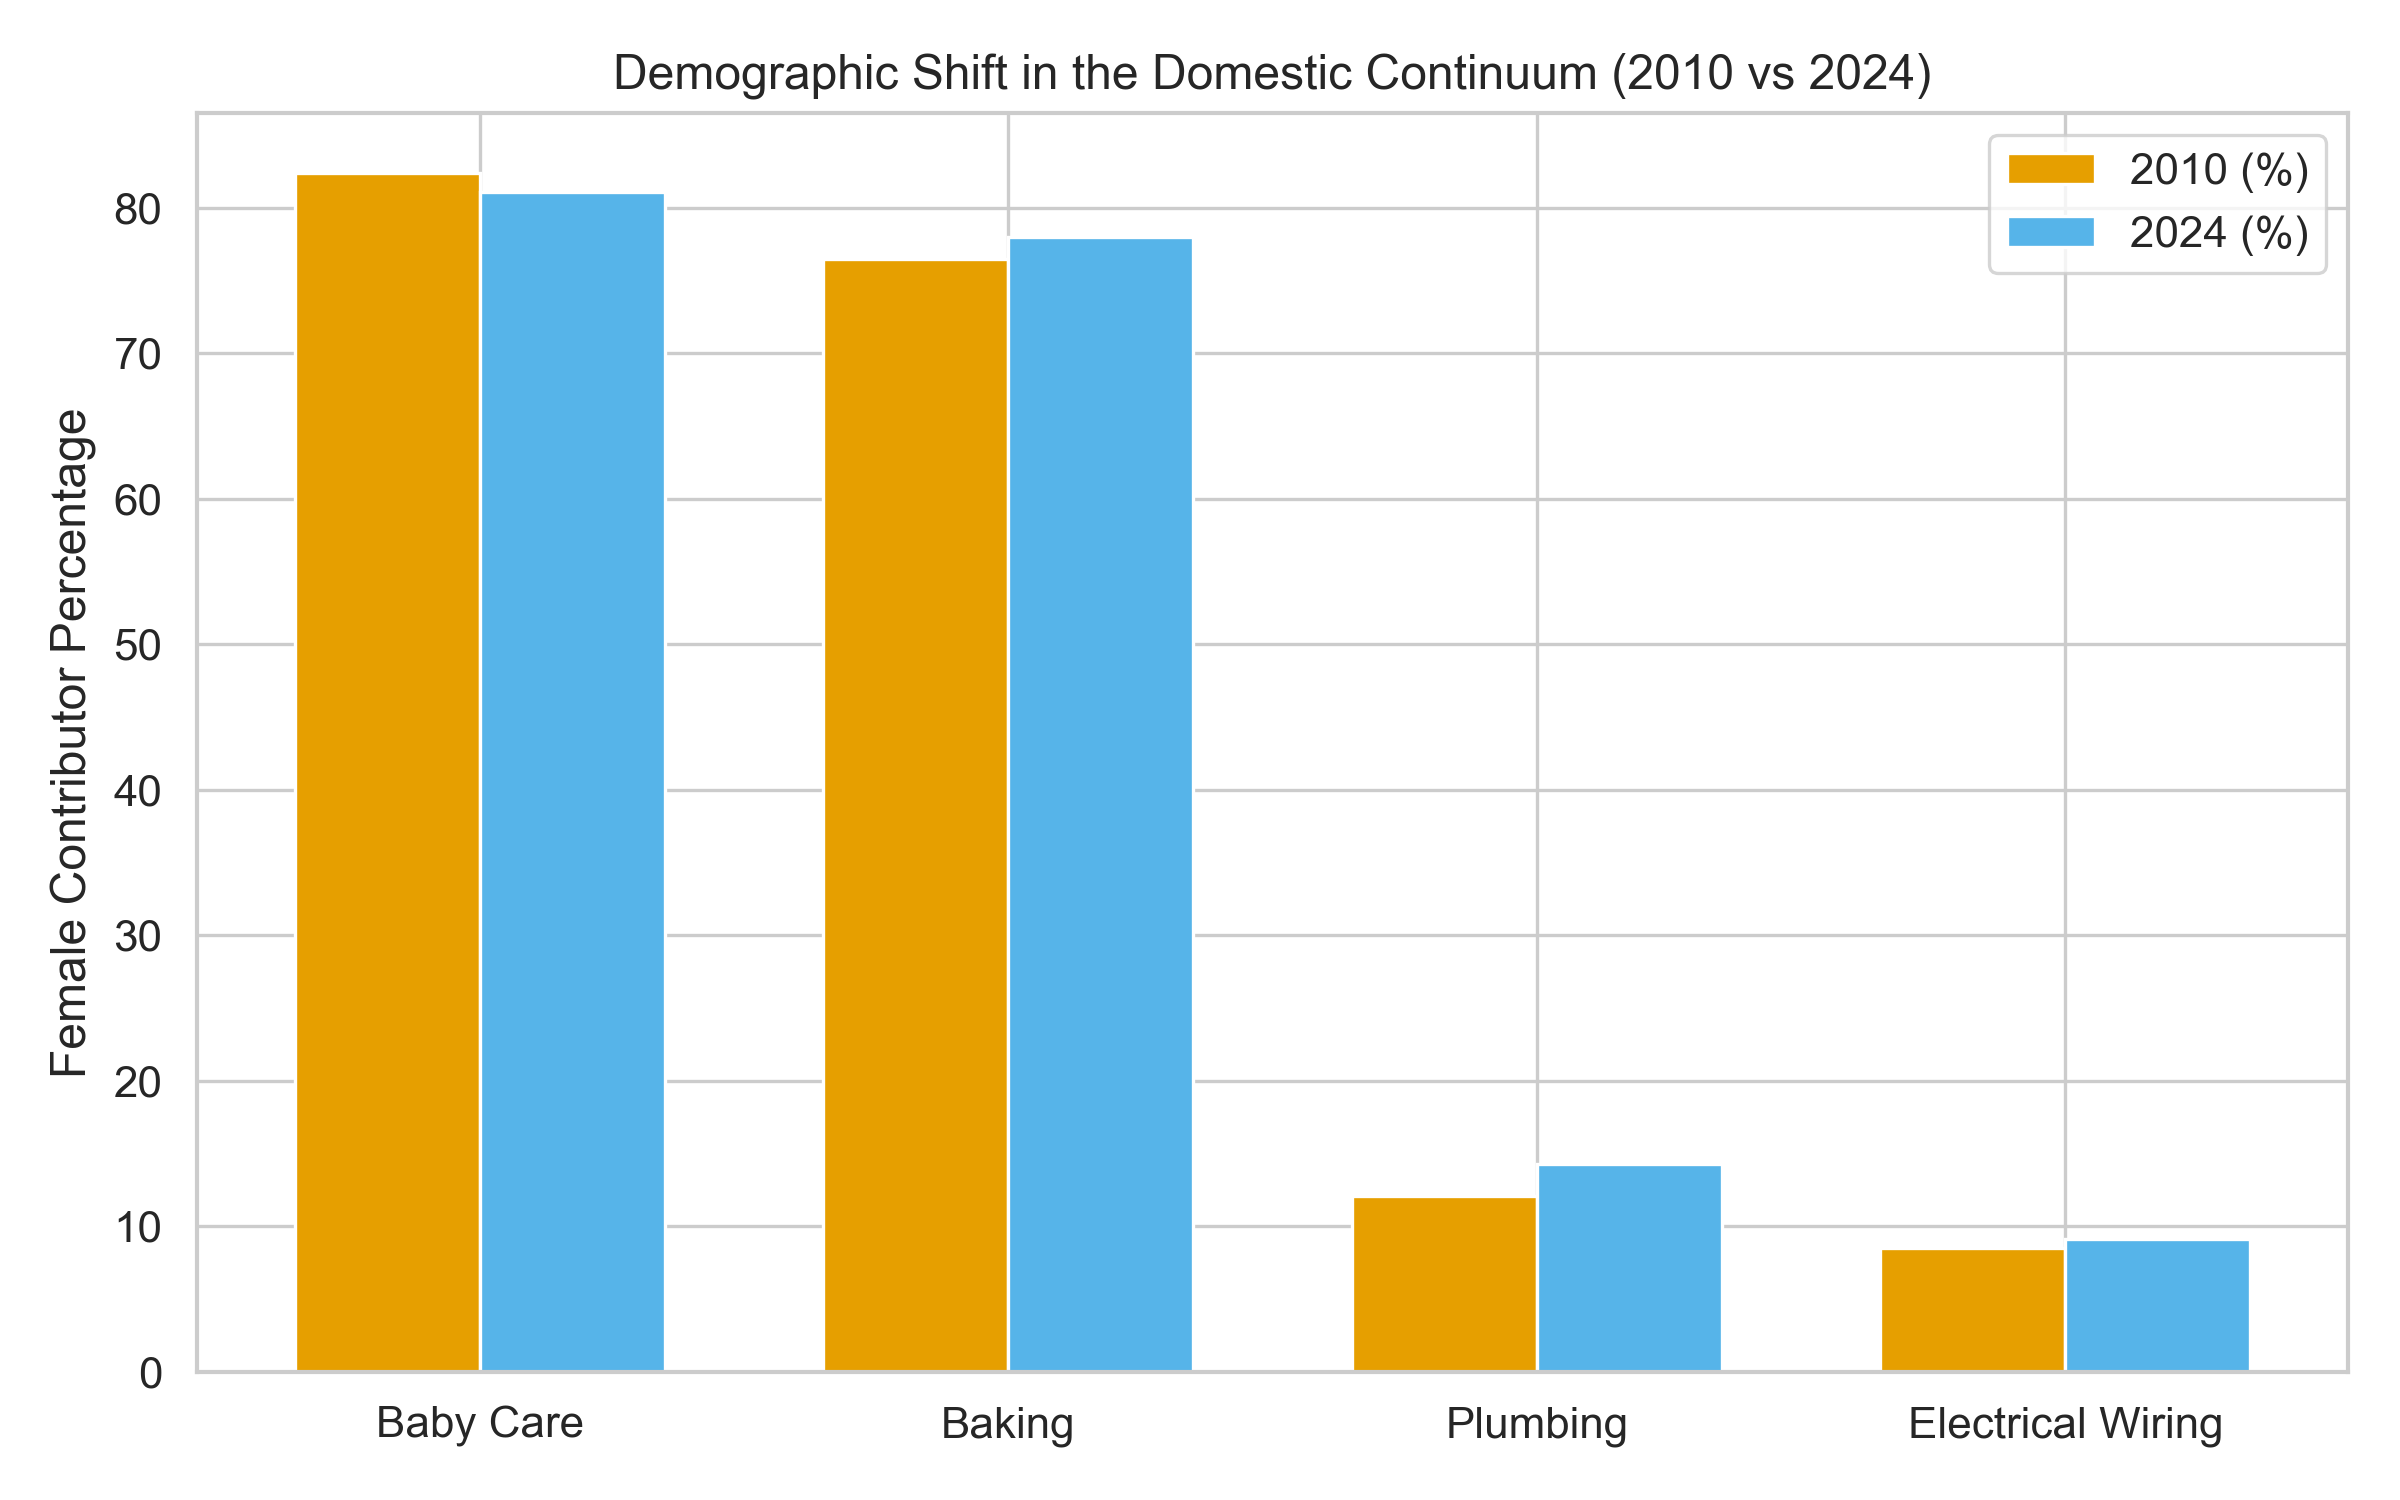
\includegraphics[width=0.8\textwidth]{images/demo_shift.png}
\caption{Projected Demographic Shift (2010 vs 2024) across the Domestic Continuum.}
\label{fig:demo_shift}
\end{figure}

\subsection{Hypothesis 2: Behavioral Profiles of Language Evolution}
Who introduces gender-neutral language, and who removes it? We project that attempts to transition articles to neutral orientations (e.g., changing ``he'' to ``they'') are predominantly initiated by Casual Users, while reverting these changes is disproportionately enforced by established Super-Users.

\begin{figure}[h]
\centering
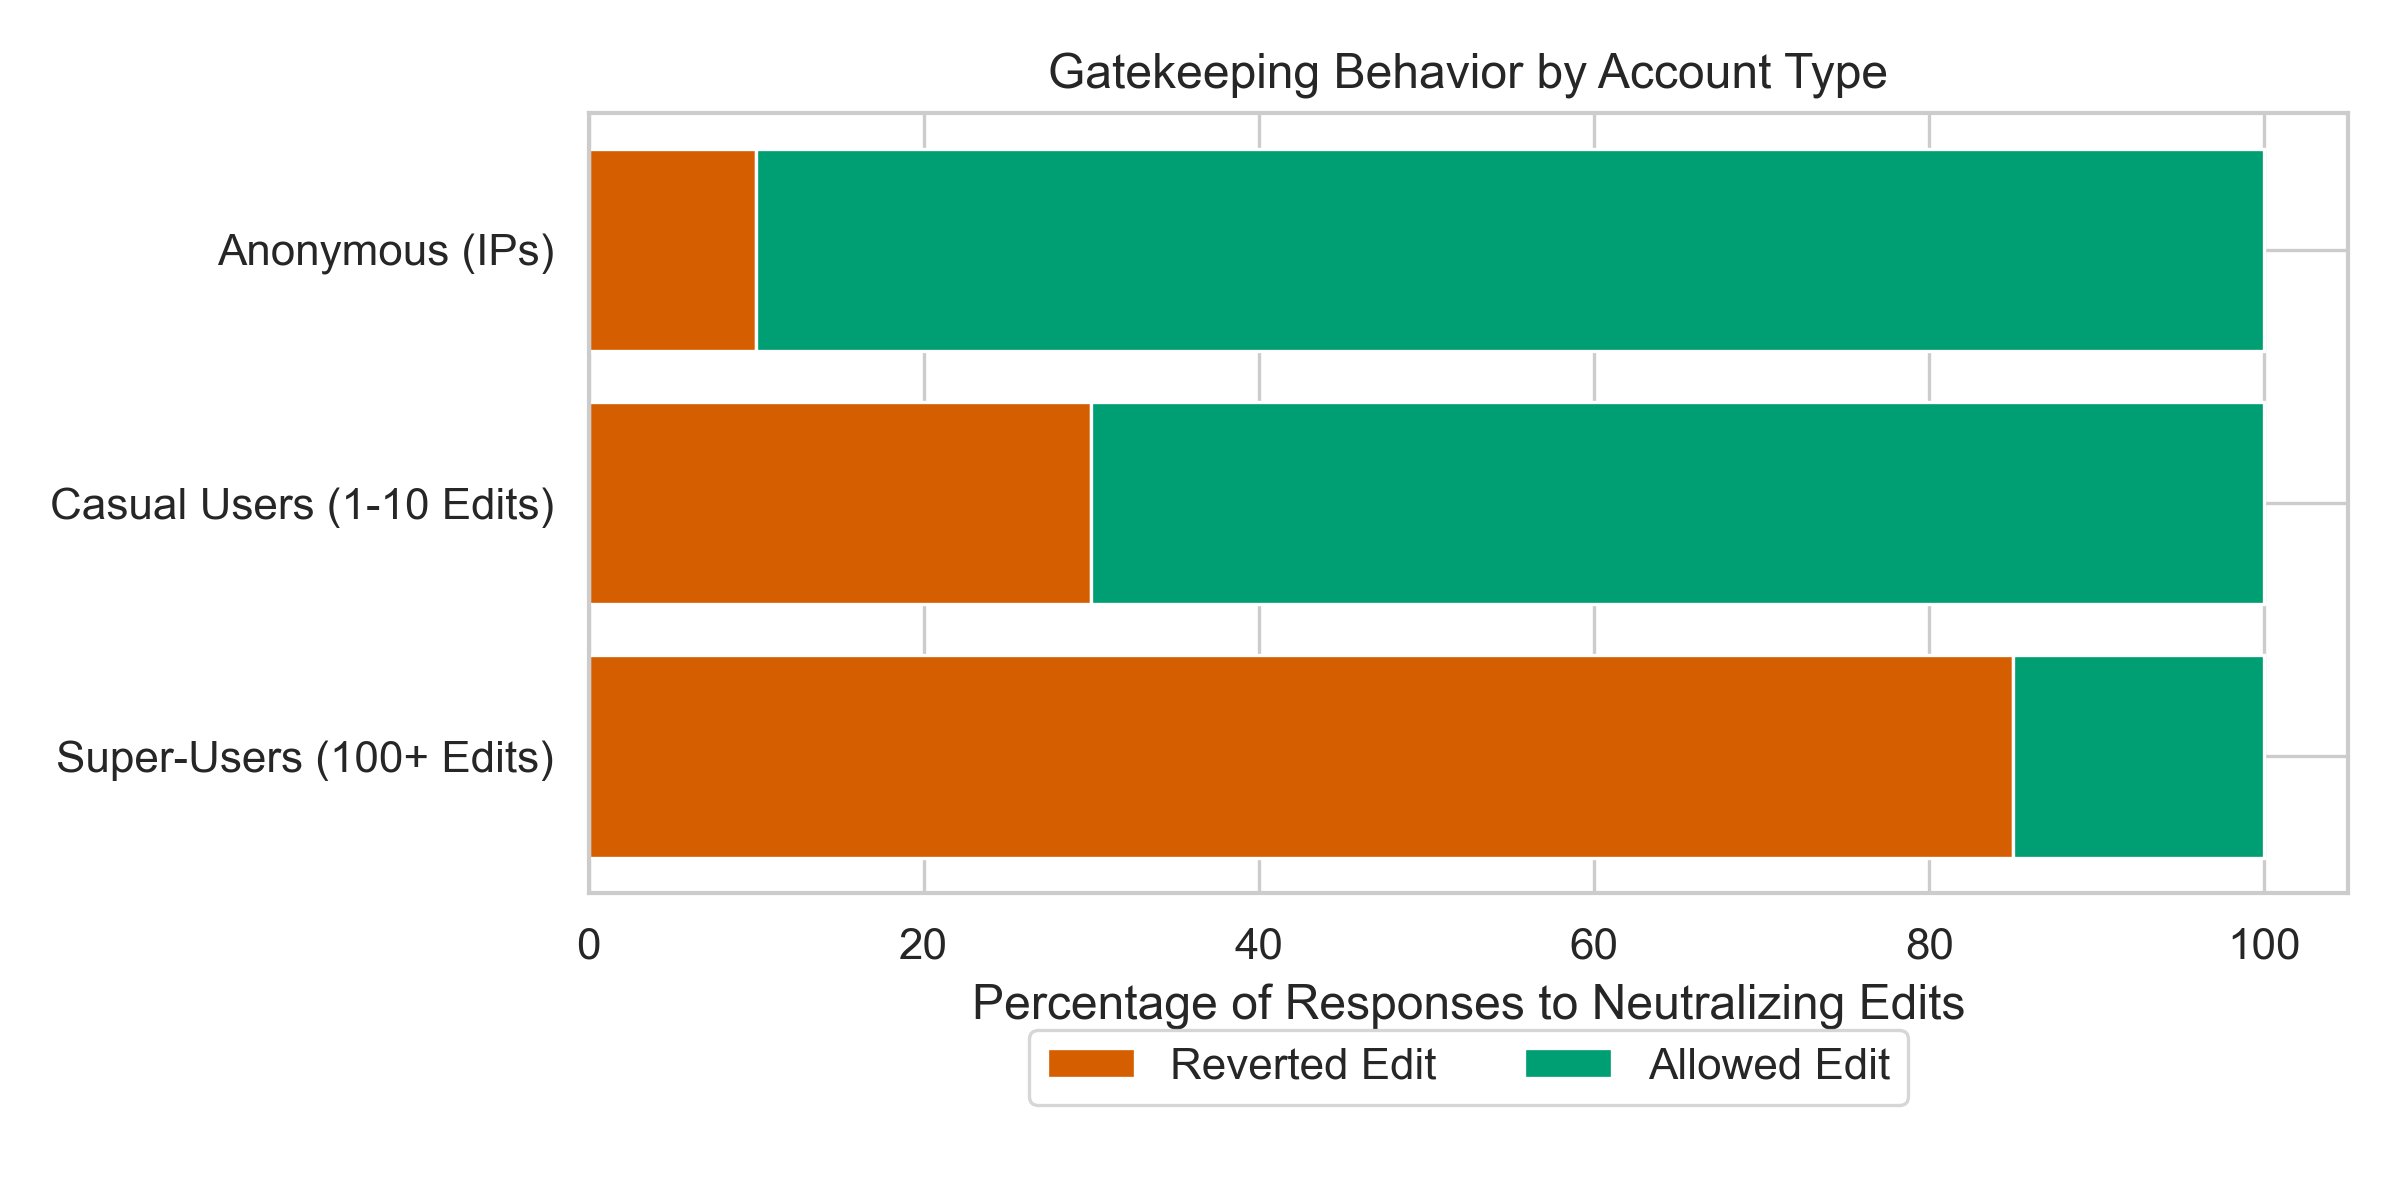
\includegraphics[width=0.85\textwidth]{images/gatekeeping.png}
\caption{Behavioral Responses to Gender-Neutralizing Edits Clustered by Account Authority.}
\label{fig:gatekeeping}
\end{figure}

\subsection{Hypothesis 3: Distinguishing Vandalism, Toxicity, and Tone Policing}
To ensure data integrity, the study maps the ratio of standard vandalism versus genuine ideological gatekeeping across the continuums. Furthermore, by analyzing the content of the vandalism itself, we hypothesize a ``Toxicity and Tone Divergence.'' We project that female-coded domains (e.g., Personal Care, Domestic) will attract disproportionately higher rates of targeted sexist trolling, body-shaming, and patronizing/moralizing edits, whereas male-coded technical domains will primarily attract generic spam or nonsensical trolling.

\begin{figure}[h]
\centering
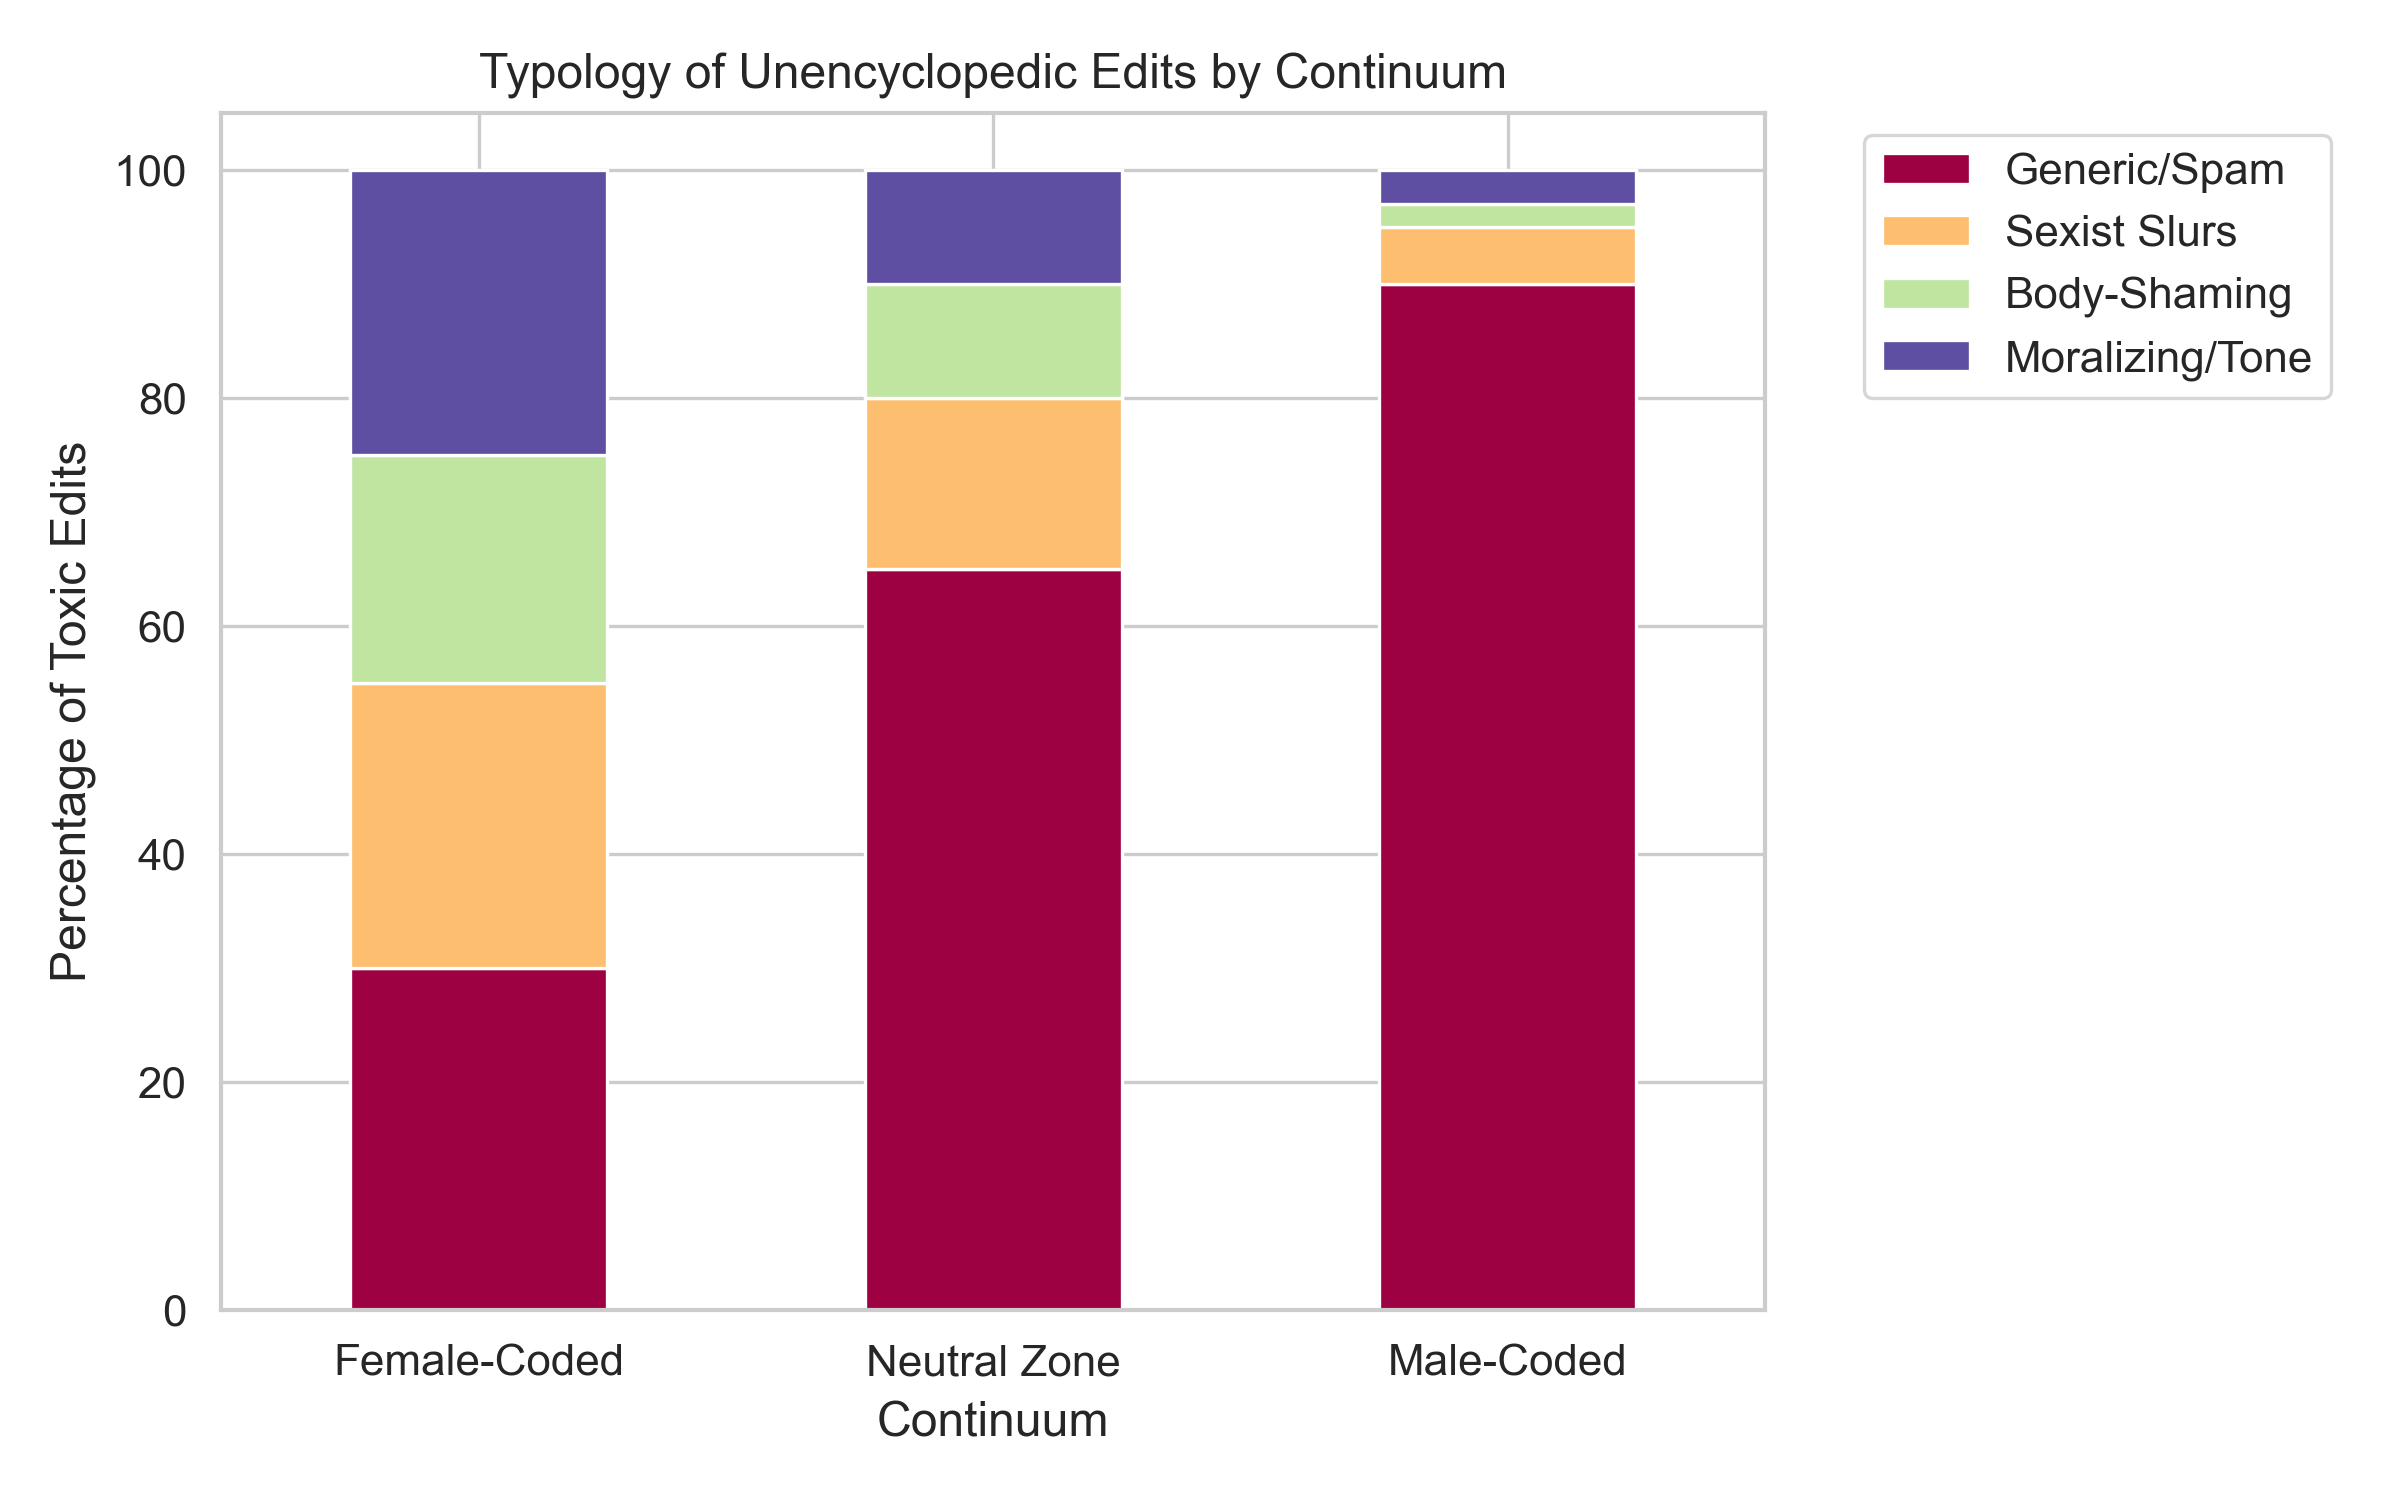
\includegraphics[width=0.9\textwidth]{images/toxicity.png}
\caption{Projected Typology of Unencyclopedic Edits, Revealing Tone and Toxicity Divergence by Continuum.}
\label{fig:toxicity}
\end{figure}

\subsection{Hypothesis 4: High-Contestation Hotspots}
Finally, the dataset will highlight the specific articles acting as cultural battlegrounds. We project that the highest raw counts of ideological edit wars will occur at the masculine extremes of Continuum 2 (Occupational Fields), specifically in \textit{Software} and \textit{Engineering}. 

\begin{table}[h]
\centering
\caption{Projected Top 5 Articles with Highest Ideological Gender Reverts}
\begin{tabular}{>{\raggedright\arraybackslash}p{4.5cm} p{3cm} c p{4.5cm}}
\toprule
\textbf{Article Title} & \textbf{Category (Pos)} & \textbf{Reverts} & \textbf{Primary Linguistic Conflict} \\
\midrule
How to Code in Python & Software (7) & 142 & Neutralizing 'he' to 'they' \\
How to Build a PC & Engineering (8) & 118 & Replacing 'craftsman/guys' \\
How to Negotiate Salary & Business (5) & 95 & Debating 'businessman' vs 'person' \\
How to Wire a Breaker & Electrical (9) & 88 & Neutralizing 'repairman' \\
How to Invest in Stocks & Pol. \& Govt. (9) & 74 & Replacing 'he/him' in examples \\
\bottomrule
\end{tabular}
\end{table}

\section{Limitations and Future Work}
This project limits its scope to the variable of gender. A primary limitation is the reliance on inferred gender when explicit pronouns are unavailable. Future work will expand this scalable pipeline to incorporate geographic metadata and advanced Word Embeddings for deeper semantic filtering.

\end{document}